% !TeX spellcheck = es_ES
\documentclass[oneside,letter,spanish,activeacute,english,links,10pt]{amcaGCS_EDO}
%\usepackage[letterpaper]{geometry}
\usepackage{graphicx}
%\usepackage{subcaption}
%\usepackage[latin1]{inputenc}
\usepackage{amsmath,amstext,amsfonts,amssymb,amsbsy,amscd,mathrsfs,array}
\usepackage{multirow,xcolor,enumerate,float}
\linespread{1.0}
% Utilidades matematicas
\newcommand{\A}{\mathbf{A}}
\newcommand{\B}{\mathbf{B}}
\newcommand{\C}{\mathbf{C}}

\newcommand{\DD}{\mathbf{D}}
\newcommand{\GG}{\mathbf{G}}
\newcommand{\Q}{\mathbf{Q}}
\newcommand{\n}{\mathbf{n}}
\newcommand{\xx}{\mathbf{x}}
\newcommand{\uu}[1][H]{\ensuremath{u_{_\mathrm{#1}}}}
\newcommand{\VV}{\mathscr{V}}
\newcommand{\VVH}[1][H]{\mathscr{V}_{\mathrm{#1}}}
\newcommand{\dOmega}{{\rm{d{\scriptstyle\Omega}}}}
\newcommand{\fin}{\hfill\rule{2mm}{3mm}}%%%%%%FIN
\newcommand{\sen}{\mbox{sen\,}}
\newcommand{\ds}[1]{\mbox{$\textstyle\displaystyle{#1}$}}

%\addto\captionsspanish{%
%	\def\bibname{Referencias}%
%	\def\tablename{Cuadro}%
%}

%%%%%%%%%%%%%%%%%%%%
% AMBIENTES DE TEOREMAS -------------------------------------------------------------------
% \newtheorem{nombre}[contador]{texto}[chapter o section]
  \newtheorem{teo}{Teorema}
  \newtheorem{cor}[teo]{Corolario}
  \newtheorem{lema}[teo]{Lema}
  \newtheorem{propo}[teo]{Proposición}
  \newtheorem{defi}{Definición}[section]
  \newtheorem{observacion}{Observación}
  \newtheorem{ejemplo}{Ejemplo}
 \newcommand{\ejem}[1]{\begin{ejemplo}{\rm {#1}}\end{ejemplo}}
 \newcommand{\teorema}[1]{\begin{teo}{#1}\end{teo}}
%\newcommand{\ds}{\displaystyle}
%\renewcommand\displaystyle{ds}
\newtheorem{defii}{Problema}
\newcommand{\pro}[1]{\begin{defii}{\rm {#1}}\end{defii}}
\providecommand{\smallpencil}{}% vacío si la instalación no lo define
\newcommand{\dirfig}{figuras/}
%\renewcommand{\tablename}{Tabla}

%%%%%%%%%%%%%%%%%%%%%%%%%%%%%%%%%%%%%%%%%%%%%%%%%%%%%%%%%%%%%%%%%%%%%%%%%%
%%%%%%%%%%%%%%%%%%%%%%%%%%%%%%%%%%%%%%%%%%%%%%%%%%%%%%%%%%%%%%%%%%%%%%%%%%
\title{ACTIVIDAD: Modelado e Inferencia de Parámetros en el Vaciado de Tanques mediante la Ley de Torricelli}
%\author[a,0]{Profesor: Giovanni Calderón}
\author[a]{Profesor: Giovanni Calderón\thanks{Notas de clases usadas para el curso de Ecuaciones Diferenciales Ordinarias.} 
	\thanks{Material disponible en el repositorio:\url{https://giovannicalderon.github.io/cursos-matematicos/}}
	\thanks{Revisiones o comentarios sobre el material es bienvenido a: \url{gecs.clase@gmail.com}}}

%
%
%\affil[a]{Escuela de Matemáticas, Facultad de Ciencias, Universidad Industrial de Santander, Bucaramanga, Colombia. 
%	
%	e-mail: \url{giovanni.calderon@correo.uis.edu.co}}


\usepackage{fancyhdr}
\pagestyle{fancy}
\setlength{\headheight}{13.6pt}
\fancyhf{}
\lhead[\leftmark]{G. Calderón}
\rhead[]{Actividad 3: Vaciado de tanques ~~~~\thepage.}
%\lfoot[\thepage]{}
%\rfoot[]{\thepage}




%\usepackage[papersize={215mm,277mm},lmargin=2.5cm,rmargin=3.5cm,top=3cm,bottom=2.5cm]{geometry}


\begin{document}

\maketitle
%\selectlanguage{spanish}
\noindent\hrulefill
\renewcommand{\abstractname}{Resumen}

\begin{abstract}
En esta actividad se modela el vaciado de un tanque cilíndrico mediante la ley de Torricelli y se plantea el problema inverso asociado: a partir de mediciones del nivel del agua en función del tiempo, estimar el radio efectivo del orificio de descarga. La solución analítica del modelo se linealiza mediante el cambio de variable $y=\sqrt{h}$, lo que permite estimar los parámetros por mínimos cuadrados. El radio estimado se interpreta físicamente en términos de una posible obstrucción del orificio, y el modelo ajustado se valida comparándolo con los datos y con una solución numérica de la ecuación diferencial.
	
	
	\bigskip\noindent{\bf Palabras clave:}
	Ecuaciones diferenciales ordinarias de primer orden, ecuaciones separables, Ley de Torricelli, vaciado de tanques, problema inverso, mínimos cuadrados.
	\\\noindent\rule[2mm]{16cm}{1pt}
	
	%\vfill
	%{\footnotetext[2]{Escuela de Matemáticas, Facultad Ciencias, Universidad Industrial de %Santander, Bucaramanga, Colombia.}}
%	{\footnotetext[0]{Notas de clases usadas para el curso de Ecuaciones Diferenciales Ordinarias. }}
	
\end{abstract}

\vspace{.6cm}


\selectlanguage{spanish}
\ifdefined\decimalpoint\decimalpoint\fi
%\pagestyle{myheadings}
%\markright{Izq}{der}
%\renewcommand{\tablename}{Tabla}

%\renewcommand{\contentsname}{Contenido del Taller:}
%\tableofcontents

\section{Introducción}
La {\it ley de Torricelli}\footnote{Evangelista Torricelli (Faenza, en la actual Italia, 1608--Florencia, 1647) fue un físico y matemático italiano. Se le atribuye la invención del barómetro. Asimismo, sus aportaciones a la geometría fueron determinantes en el desarrollo del cálculo integral.} establece que la velocidad de salida de un líquido por un orificio en un recipiente es igual a la que alcanzaría un cuerpo en caída libre desde la superficie del líquido hasta dicho orificio \cite{Boyce, Zill1, Zill2, FoxMcDonald2015}. Esta ley se deduce de la aplicación del principio de Bernoulli a fluidos ideales bajo la acción de la gravedad.

En esta actividad se estudia el vaciado de un tanque por un orificio mediante un balance de volumen y la ley de Torricelli, con el propósito de construir un modelo matemático que describa la evolución del nivel del líquido en el tiempo. A diferencia del enfoque directo, en el que se calcula la solución a partir de parámetros conocidos, aquí se considera también el problema inverso: utilizar mediciones del nivel del agua para estimar un parámetro hidráulico del sistema que no se observa directamente.

Este tipo de análisis tiene interés en sistemas reales de almacenamiento de agua, como los tanques de las redes contra incendios, cuyo diseño se rige por normas como la NFPA 22 \cite{NFPA2024, IFP2024}. En estos sistemas, las incrustaciones, el desgaste o la acumulación de sedimentos pueden modificar el área efectiva del orificio de descarga y alterar el comportamiento hidráulico esperado. Por ello resulta útil contar con modelos que permitan inferir propiedades físicas del sistema a partir de datos experimentales.

El objetivo de esta actividad es estudiar el modelo diferencial correspondiente, obtener su solución analítica, utilizar datos de nivel para estimar parámetros mediante técnicas de ajuste e interpretar físicamente los resultados. Para ello se emplearán herramientas computacionales (Python o MATLAB) que permitan visualizar el comportamiento del modelo y explorar su sensibilidad frente a variaciones en los parámetros.

\section{Problema Modelo}
Considere un tanque cilíndrico vertical utilizado para almacenar agua en un sistema de protección contra incendios (ver Figura \ref{fig:1})\footnote{Los tanques cilíndricos verticales utilizados en sistemas contra incendios suelen diseñarse conforme a la norma NFPA 22.}. Durante una prueba de mantenimiento, el tanque se vacía parcialmente a través de una tubería de descarga ubicada en la pared lateral, junto al fondo, mientras un sensor registra el nivel del agua en función del tiempo.
\begin{figure}[!h]
	\centering
	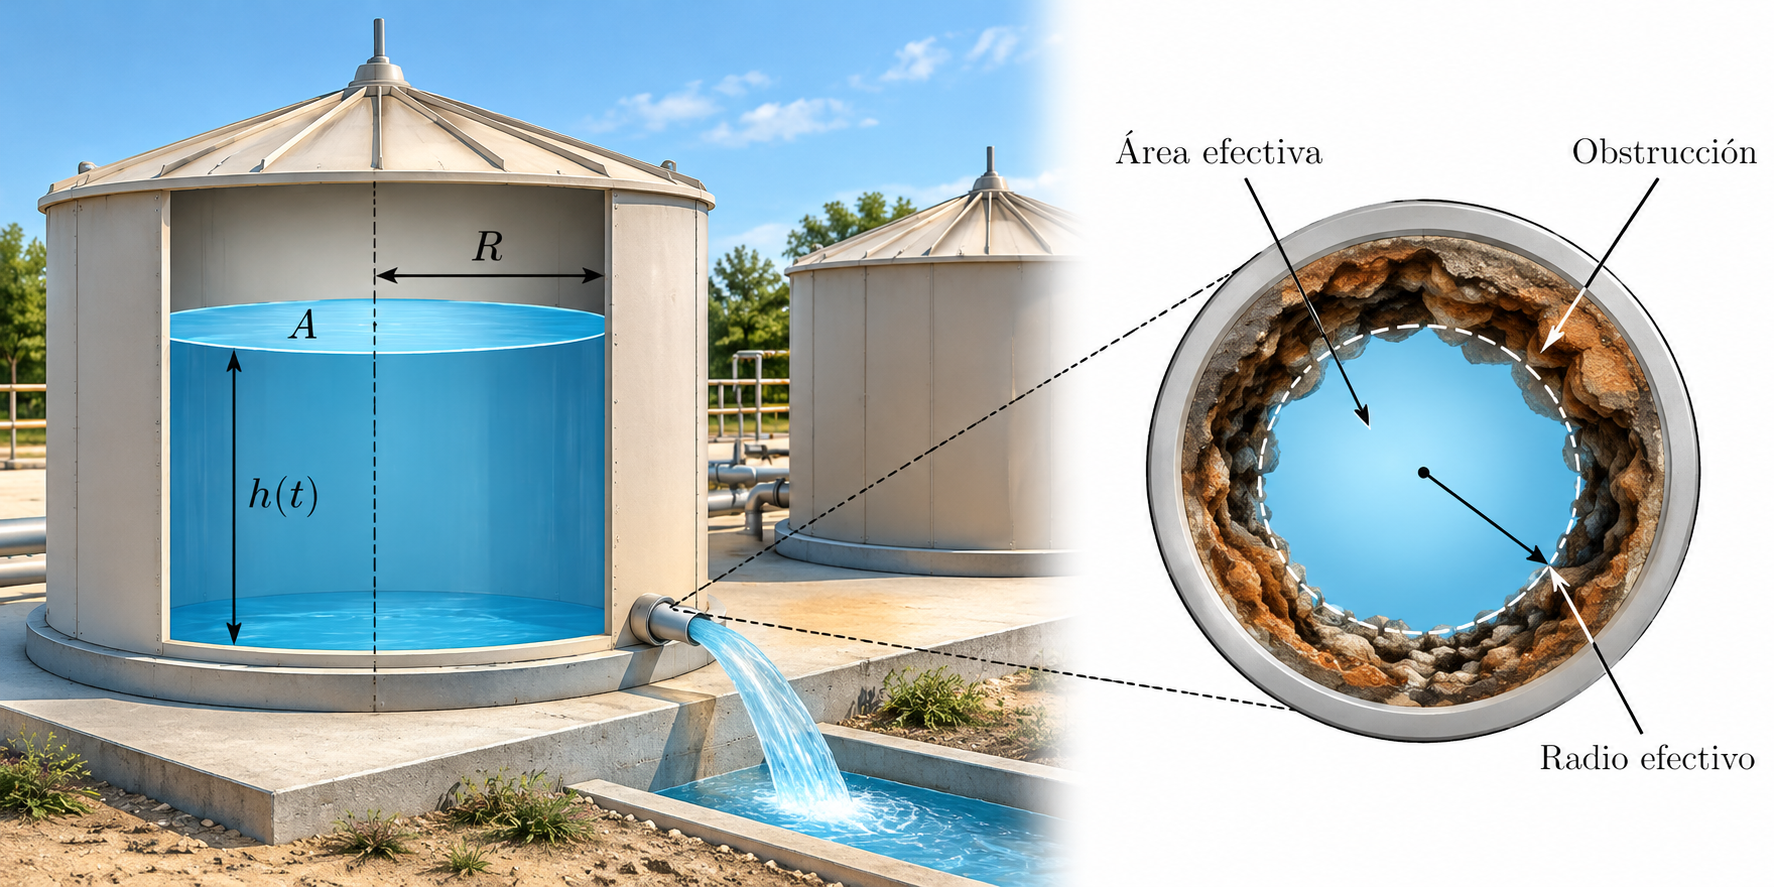
\includegraphics[scale=0.2]{Figuras/EsquemaTanqueTuberiaCorroida.png}
	\caption{Tanque cilíndrico de almacenamiento de agua con descarga lateral junto al fondo. Ampliación: sección de la tubería de descarga con incrustaciones que reducen el área libre de paso. Imagen ilustrativa generada con inteligencia artificial; no está a escala.}\label{fig:1}
\end{figure}

El tiempo de vaciado depende de la geometría del tanque y del orificio de descarga. Con el uso continuo pueden presentarse incrustaciones, sedimentos o desgaste que modifican el área libre de paso del orificio (ver la ampliación de la Figura \ref{fig:1}). Como esa área es difícil de medir directamente, interesa estimarla a partir del comportamiento observable del sistema. Para describir el área de paso, aun cuando no sea circular, se utiliza el \emph{radio efectivo} $r$: el radio del círculo cuya área coincide con el área libre de paso.

Sea $h(t)$ la altura del agua sobre el centro del orificio de descarga en el instante $t$. Como el orificio está junto al fondo, $h$ coincide prácticamente con la altura del agua en el tanque. Si $A_w$ es el área de la superficie libre y $Q(t)$ es el caudal de salida, el balance de volumen establece que
$$
A_w\,\frac{dh}{dt}=-Q .
$$
La ley de Torricelli da la velocidad de salida $v=\sqrt{2gh}$. Debido a la contracción del chorro y a las pérdidas por fricción, el caudal real es $Q=C_d\,A_h\sqrt{2gh}$, donde $C_d<1$ es el coeficiente de descarga. Sustituyendo, se obtiene
\begin{equation}\label{ec1}
	\frac{d h}{d t}=-C_d \frac{A_h}{A_w} \sqrt{2 g h},
\end{equation}
donde
\begin{itemize}
	\item $h(t)$ es la altura del agua sobre el centro del orificio (m),
	\item $A_h=\pi r^2$ es el área efectiva del orificio de descarga (m$^2$) y $r$ su radio efectivo (m),
	\item $A_w=\pi R^2$ es el área de la sección transversal del tanque (m$^2$), constante en un tanque cilíndrico de radio $R$ (m),
	\item $C_d$ es el coeficiente de descarga (adimensional),
	\item $g$ es la aceleración de la gravedad (m/s$^2$).
\end{itemize}
El modelo supone un fluido incompresible, un flujo cuasiestacionario (la superficie libre desciende lentamente porque $A_h\ll A_w$) y un coeficiente de descarga constante durante el vaciado.

La ecuación diferencial \eqref{ec1} es separable. Con la condición inicial $h(0)=h_0$, su solución satisface
$$
\sqrt{h(t)}=\sqrt{h_0}-\frac{1}{2} C_d \frac{r^2}{R^2} \sqrt{2 g}\, t ,
$$
o, de manera equivalente,
\begin{equation}\label{ec2}
	h(t)=\left(\sqrt{h_0}-\frac{1}{2} C_d \frac{r^2}{R^2} \sqrt{2 g}\, t\right)^2 .
\end{equation}
Esta expresión describe la evolución del nivel del agua y permite calcular tiempos característicos del vaciado. Debe tenerse en cuenta que solo es válida en un intervalo de tiempo finito (véase el ítem 1(a) de la actividad).

Para el tanque bajo estudio se tienen los valores del Cuadro \ref{tab:parametros}.
\begin{table}[h]
	\centering
	\begin{tabular}{lll}
		\hline
		Parámetro & Descripción & Valor (unidades) \\
		\hline
		$r_0$ & radio nominal del orificio (sin obstrucción) & $0.04$ m \\
		$R$   & radio del tanque              & $2.5$ m \\
		$C_d$ & coeficiente de descarga esperado      & $0.61$ (adimensional) \\
		$g$   & aceleración de la gravedad  & $9.81$ m/s$^{2}$ \\
		$h_0$ & altura inicial del agua sobre el orificio & $10.0$ m \\
		\hline
	\end{tabular}
	\caption{Parámetros del tanque cilíndrico.}\label{tab:parametros}
\end{table}

Durante la prueba de drenaje se registraron los niveles del Cuadro \ref{tab:datos_altura}. Estos datos son sintéticos: se generaron con el modelo \eqref{ec2} para un radio efectivo conocido por el docente y se redondearon a dos cifras decimales, lo que reproduce la resolución finita (0.01 m) de un sensor de nivel. No contienen otras fuentes de error, de modo que permiten evaluar qué tan bien se recupera el parámetro cuando la única perturbación es la resolución de la medida.
% NOTA (pendiente de decisión del autor): con r = 0.035 m, Cd = 0.61, g = 9.81 m/s^2
% y h0 = 10 m, el modelo da h(2400) = 6.3846 m, que redondea a 6.38 y no a 6.39.
% El mismo valor aparece en el artículo; decidir allí y aquí de forma coherente.
\begin{table}[H]
	\centering
	\small
	\setlength{\tabcolsep}{4pt}\renewcommand{\arraystretch}{1.3}
	\begin{tabular}{c|ccccccccccccc}
		\hline\\[-12pt]
		$t$ (s)
		& 0 & 300 & 600 & 900 & 1200 & 1500 & 1800 & 2100 & 2400 & 2700 & 3000 & 3300 & 3600 \\
		\hline\\[-12pt]
		$h$ (m)
		& 10.00 & 9.50 & 9.02 & 8.55 & 8.09 & 7.65 & 7.21 & 6.79 & 6.39 & 5.99 & 5.61 & 5.24 & 4.88\\
		\hline
	\end{tabular}
	\caption{Mediciones sintéticas del nivel del agua, redondeadas a dos cifras decimales.}\label{tab:datos_altura}
\end{table}

\subsection{Linealización del modelo}
De la solución \eqref{ec2} se sigue que la variable $y(t)=\sqrt{h(t)}$ satisface una relación lineal en el tiempo,
\begin{equation}\label{ec3}
	y(t)=\sqrt{h_0}-\beta t ,
\end{equation}
donde
\begin{equation}\label{ec4}
	\beta=\frac{1}{2} C_d \frac{r^2}{R^2} \sqrt{2 g}.
\end{equation}
Así, en el plano $(t,y)$ los datos deben alinearse sobre una recta de pendiente $-\beta$ y ordenada en el origen $\sqrt{h_0}$. La pendiente estimada por mínimos cuadrados proporciona $\beta$ y, despejando $r$ de \eqref{ec4}, se obtiene el radio efectivo del orificio. Observe que los datos determinan $C_d$ y $r$ solo a través del producto $C_d\,r^2$; por eso, para estimar $r$ se adopta el valor esperado $C_d=0.61$ del Cuadro \ref{tab:parametros}.

\subsection{Objetivo del análisis}
El propósito del análisis es utilizar los datos disponibles para estimar los parámetros del modelo y evaluar su significado físico. En particular, se busca:
\begin{itemize}
	\item estimar el parámetro $\beta$,
	\item calcular el radio efectivo del orificio,
	\item comparar el radio estimado con el valor nominal,
	\item interpretar las posibles causas físicas de las diferencias observadas.
\end{itemize}
Este procedimiento permite evaluar si el sistema hidráulico se comporta de acuerdo con las condiciones esperadas o si hay evidencia de alteraciones físicas como obstrucciones o desgaste.

\section{Actividad a realizar}
Todos los resultados numéricos deben expresarse con sus unidades físicas y con una cantidad razonable de cifras significativas. Indique claramente las unidades del parámetro $\beta$ y del radio estimado $r$. Los cálculos deben realizarse con código propio, comentado y reproducible.

\begin{enumerate}
	\item {\bf Modelo y linealización.}
	\begin{enumerate}
		\item Resuelva la ecuación \eqref{ec1} por separación de variables con la condición $h(0)=h_0$ y obtenga \eqref{ec2}. Determine el intervalo de tiempo en el que \eqref{ec2} describe el sistema y explique por qué deja de hacerlo fuera de él.
		\item Muestre que $y(t)=\sqrt{h(t)}$ satisface \eqref{ec3} con $\beta$ dado por \eqref{ec4}, y verifique que $\beta$ tiene unidades de m$^{1/2}$/s.
		\item Construya una nueva tabla de datos con los valores $y_i=\sqrt{h_i}$.
		\item Grafique los datos $h(t)$ y $y(t)$ y describa cualitativamente su comportamiento. ¿Por qué la rapidez de descenso del nivel disminuye a medida que el tanque se vacía?
	\end{enumerate}
	
	\item {\bf Estimación del parámetro $\beta$.}
	Utilizando los datos transformados:
	\begin{enumerate}
		\item Plantee las ecuaciones normales del ajuste por mínimos cuadrados del modelo lineal $y=a+m t$ y resuélvalas.
		\item Reporte los valores estimados de $a$ y $m$ con sus unidades.
		\item Interprete físicamente el valor estimado de $a$, compárelo con $\sqrt{h_0}$ y calcule el error relativo.
		\item Determine el valor estimado del parámetro $\beta=-m$.
		\item Grafique en una misma figura los datos transformados y la recta ajustada.
		\item Grafique los residuos $y_i-(a+m t_i)$. ¿Muestran algún patrón? ¿Es su tamaño compatible con el redondeo de $h$ a dos cifras decimales?
	\end{enumerate}
	
	\item {\bf Estimación del radio efectivo del orificio.}
	Usando la relación \eqref{ec4}:
	\begin{enumerate}
		\item Despeje algebraicamente el radio $r$ y calcule el radio efectivo estimado.
		\item Compare el valor obtenido con el radio nominal $r_0$ y determine el porcentaje de reducción del radio y el porcentaje de reducción del área del orificio.
	\end{enumerate}
	
	\item {\bf Validación del modelo.}
	Usando el radio efectivo estimado:
	\begin{enumerate}
		\item Construya la función $h(t)$ dada por \eqref{ec2}, con $h_0$ del Cuadro \ref{tab:parametros}.
		\item Grafique en una misma figura los datos, la curva del modelo ajustado y la curva que se obtendría con el radio nominal $r_0$.
		\item Calcule el error cuadrático medio $\mathrm{ECM}=\frac{1}{N}\sum_{i=1}^{N}\left(h_i-h(t_i)\right)^2$ entre los datos y el modelo ajustado, e interprete su valor.
		\item Resuelva numéricamente la ecuación \eqref{ec1} con un método de Runge--Kutta de cuarto orden (o con una rutina como \texttt{solve\_ivp} u \texttt{ode45}) y compare la solución numérica con \eqref{ec2} en el intervalo de los datos. Explique por qué conviene detener la integración antes de que $h$ se anule.
		\item Determine el tiempo total de vaciado estimado y compárelo con el que tendría el tanque con el radio nominal.
	%	\item Analice cómo cambiaría el tiempo de vaciado si el radio efectivo disminuyera un 10\% adicional. Justifique el resultado a partir de \eqref{ec4}.
	\end{enumerate}
	
	\item {\bf Inferencia e interpretación ingenieril.}
	A partir de los resultados obtenidos:
	\begin{enumerate}
		\item Discuta si el radio efectivo estimado sugiere una obstrucción parcial, desgaste del sistema o condiciones normales de operación.
		\item Suponga que el sistema debe alcanzar una altura $h=2$ m antes de 2 horas. Determine si cumple esta condición.
		\item Suponga que el coeficiente de descarga real difiere en $\pm 5\%$ del valor asumido. Con los mismos datos, ¿cómo cambia el radio efectivo estimado? ¿Cambia el tiempo de vaciado predicho? Explique el resultado a partir de \eqref{ec4}.
		\item Proponga qué información experimental adicional permitiría estimar simultáneamente $C_d$ y $r$ sin asumir previamente el valor de alguno de ellos. Justifique su respuesta desde el punto de vista físico y matemático.
	\end{enumerate}
\end{enumerate}


\section{Instrucciones para la actividad}
Tenga presentes las siguientes instrucciones al momento de entregar el informe:
\begin{itemize}
	\item La actividad se realizará en grupo y el informe se debe elaborar en un cuaderno de Google Colab con el nombre
	\verb+Act3_Vaciado_B2_NombreApellido.ipynb+,
	que se debe COMPARTIR con el usuario \verb+gecs.clase@gmail.com+.
	En el nombre del archivo, \verb+B2+ indica el grupo del curso (A4, A5, B2 o E1) y \verb+NombreApellido+ el nombre de uno de los integrantes. No se acepta otro tipo de entrega ni se revisan correos adicionales para verificar la entrega. Solo se trabaja en el directorio (Drive) de dicha cuenta de correo.
	\item En el preámbulo del informe deben aparecer los nombres completos de los integrantes y el grupo del curso al cual pertenecen.
	\item El archivo compartido en Drive debe tener permiso de edición.
\end{itemize}

\bigskip\noindent{\bf Observación:} El archivo NO DEBE enviarse por correo como archivo adjunto; debe compartirse en Drive.

\section{Rúbrica de evaluación}

La rúbrica del Cuadro \ref{tab:rubrica} evalúa la actividad considerando claridad, precisión matemática y análisis crítico.

\begin{table}[h!]
	\centering
	\footnotesize
	\renewcommand{\arraystretch}{1.25}
	\begin{tabular}{|p{2.0cm}|p{3.3cm}|p{2.8cm}|p{2.8cm}|p{2.8cm}|}
		\hline
		\textbf{Criterio}
		& \textbf{Excelente (5 puntos)}
		& \textbf{Bueno (4 puntos)}
		& \textbf{Aceptable (3 puntos)}
		& \textbf{Deficiente (2 puntos o menos)} \\
		\hline
		\textbf{Modelado Matemático}
		& Ecuaciones bien definidas, justificadas y claramente interpretadas.
		& Ecuaciones claras pero con justificación limitada.
		& Modelo funcional con errores menores.
		& Modelo incompleto o con errores graves. \\
		\hline
		\textbf{Ajuste de Parámetros}
		& Ajuste correcto con pasos claros, detallados y bien documentados.
		& Ajuste correcto pero con algunos pasos incompletos.
		& Ajuste incompleto o con errores menores.
		& Ajuste ausente o procedimiento incorrecto. \\
		\hline
		\textbf{Resolución de la EDO}
		& Solución analítica y numérica correctas, justificadas y comparadas con gráficos claros.
		& Resolución correcta pero con algunos detalles faltantes.
		& Resolución incompleta o con errores menores.
		& Resolución ausente o incorrecta. \\
		\hline
		\textbf{Análisis de Resultados}
		& Análisis profundo con interpretación matemática clara y coherente con el modelo.
		& Análisis adecuado pero con interpretación limitada.
		& Análisis incompleto o con poca claridad conceptual.
		& Sin análisis o con interpretación incorrecta. \\
		\hline
		\textbf{Interpretación Física}
		& Resultados interpretados correctamente dentro del contexto físico del sistema, incluyendo discusión del radio estimado y sus implicaciones.
		& Interpretación física adecuada pero con análisis limitado del contexto.
		& Interpretación superficial o incompleta del significado físico.
		& Sin interpretación física o con conclusiones incorrectas. \\
		\hline
		\textbf{Creatividad}
		& Extensión innovadora y bien fundamentada del modelo o del análisis.
		& Ideas creativas pero no completamente desarrolladas.
		& Propuestas básicas o con desarrollo limitado.
		& Sin extensiones ni propuestas novedosas. \\
		\hline
		\textbf{Presentación del Informe}
		& Estructura clara, bien organizada, sin errores gramaticales y con referencias claras al procedimiento.
		& Bien organizado pero con errores menores en redacción o estructura.
		& Desorganizado o con errores significativos en redacción.
		& Informe incompleto, desorganizado o con errores graves. \\
		\hline
		\textbf{Reglas de entrega del Informe}
		& Cumple todas las instrucciones establecidas.
		& Cumple al menos el 80\% de las instrucciones.
		& Cumple aproximadamente el 60\% de las instrucciones.
		& Cumple menos del 60\% de las instrucciones. \\
		\hline
		\textbf{Sustentación del informe}
		& Presentación clara, organizada y dentro del tiempo asignado. Resultados explicados e interpretados correctamente. Participación equilibrada del grupo y uso adecuado de gráficas o tablas.
		& Presentación comprensible pero con algunas fallas en organización o claridad. Interpretación parcial de resultados o participación desigual.
		& Presentación poco clara o desorganizada. Explicación limitada de resultados y escasa participación del grupo.
		& Presentación confusa o incompleta, sin interpretación de resultados ni organización evidente. \\
		\hline
	\end{tabular}
	\caption{Rúbrica de evaluación para la actividad de modelado del vaciado de tanques mediante la ley de Torricelli.}
	\label{tab:rubrica}
\end{table}

\begin{thebibliography}{99}
	\bibitem{Boyce} Boyce, W. E., DiPrima, R. C. \emph{Ecuaciones diferenciales y problemas con valores en la frontera}, 4.\textordfeminine\ ed., Limusa, México, 2000.
	% VERIFICAR: edición y año con la portadilla del ejemplar usado.
	
	\bibitem{Zill1} Zill, D. G., Wright, W. S. \emph{Ecuaciones diferenciales con problemas con valores en la frontera}, 8.\textordfeminine\ ed., Cengage Learning, México, 2015.
	
	\bibitem{Zill2} Zill, D. G., Wright, W. S. \emph{Matemáticas avanzadas para ingeniería}, 4.\textordfeminine\ ed., McGraw-Hill, México, 2012.
	
	\bibitem{NFPA2024}
	National Fire Protection Association.
	\newblock \textit{Tank Talk: Water Storage Tanks for Fire Protection Systems}.
	\newblock 30 de octubre de 2024.
	\newblock Disponible en:
	\url{https://www.nfpa.org/news-blogs-and-articles/blogs/2024/10/30/nfpa-22-and-water-storage-tanks}.
	\newblock Consultado el 28 de marzo de 2026.
	
	\bibitem{IFP2024}
	IFP Magazine.
	\newblock \textit{What Constitutes NFPA 22 Compliance and Equivalency?}
	\newblock 2024.
	\newblock Disponible en:
	\url{https://ifpmag.com/what-constitutes-nfpa-22-compliance-and-equivalency/}.
	\newblock Consultado el 28 de marzo de 2026.
	
	\bibitem{FoxMcDonald2015}
	Fox, R. W., McDonald, A. T., Pritchard, P. J.
	\newblock \textit{Introduction to Fluid Mechanics}.
	\newblock 9th ed., John Wiley \& Sons, 2015.
	% VERIFICAR: hasta donde se sabe, la 8.a ed. (2011) es de Fox, McDonald y Pritchard,
	% y la 9.a ed. figura como Pritchard y Mitchell, "Fox and McDonald's Introduction to
	% Fluid Mechanics". Ajustar autores y título según el ejemplar consultado.
\end{thebibliography}

\end{document}




